\documentclass[11pt,a4paper]{scrreprt}

\usepackage[utf8]{inputenc}
\usepackage[italian]{babel}

\usepackage{amsmath, amsfonts}
\usepackage{graphicx}

\usepackage{parskip}
\usepackage{color}

\usepackage{placeins}

\usepackage{url}

\newtheorem{teorema}{Teorema}
\newtheorem{lemma}[teorema]{Lemma}
\newtheorem{proposizione}[teorema]{Proposizione}
\newtheorem{proprieta}[teorema]{Proprietà}

\author{L. De Sano, A. Donizetti}
\title{\textsc{FIC}: Fractal Image Compression}
\date{Settembre 2015}

\begin{document}
\maketitle

\tableofcontents

\chapter{Introduzione}

Con il termine ``Fractal image Compression'' si va ad indicare una famiglia di tecniche di compressione di immagini (o video) basate sulle proprietà matematiche dei frattali. Tali metodi di compressione si rivelano sopra ogni altra cosa adatti a comprimere textures e immagini naturali, o, più in generale, immagini che sono caratterizzate da un elevato livello di \emph{self-similarity} (ovvero aventi delle parti che, al netto di rotazioni e ingrandimenti/riduzioni, somigliano ad altre parti dell'immagine).

La compressione di immagini tramite frattali (così come altre, più diffuse, ad esempio \textit{JPEG}) appartiene a quel gruppo di tecniche di compressione \emph{lossy}, ovvero in cui la compressione dell'immagine avviene al costo di una perdita di informazione. Tuttavia, a differenza di quanto accade quando si utilizza uno dei metodi di compressione basati sui pixel (come \textit{JPEG}, \textit{GIF} o \textit{MPEG}), nella compressione frattale nessuna parte dell'immagine viene effettivamente memorizzata. Ciò che viene memorizzato è invece la \emph{struttura interna} dell'immagine (ad esempio un indice di quali parti, effettuate le dovute trasformazioni, sono simili ad altre parti). 

Poiché nessun pixel dell'immagine originale viene memorizzato, la decompressione parte da un singolo pixel, di colore qualsiasi, e procede alla ricostruzione dell'immagine originale applicando iterativamente una mappa ricavata dalla struttura interna dell'immagine originale.

In questo documento tratteremo delle tecniche di compressione di immagini basate su frattali, iniziando con una panoramica teorica del loro funzionamento, proseguendo con la discussione di alcuni aspetti pratici e presentando una implementazione giocattolo realizzata in MATLAB, e concludendo infine con alcuni test che consentiranno di valutare praticità e \emph{performances} di una libreria di compressione basata su frattali, anche in confronto con altre tecniche di compressione \emph{lossy} maggiormente utilizzate.

\chapter{Aspetti teorici}

\section{Introduzione ai frattali}

Un frattale è un oggetto geometrico che si ripete nella sua forma, allo stesso modo, su diverse scale. Questo comportamento fa si che ingrandendo una sua qualsiasi componente, ciò che si ottiene è una figura simile all'originale. In linea di massima, si può dire che perché l'insieme $F$ sia considerato un frattale, $F$ dovrebbe avere almeno le seguenti proprietà:

\begin{itemize}
\item $F$ ha dettagli ad ogni scala d'ingrandimento;
\item $F$ gode di autosimilitudine (a qualunque scala si osservi, presenta sempre le stesse caratteristiche globali);
\item la dimensione frattale di $F$ è maggiore della sua dimensione topologica;
\item esiste un algoritmo relativamente semplice per costruire $F$.
\end{itemize}

{\color{red} TODO: definire dimensione frattale e topologica}

\url{http://www.vanderbilt.edu/AnS/psychology/cogsci/chaos/workshop/Fractals.html}

% mettere qualche esempio di frattale di base con la costruzione iterata?

Un esempio di oggetto geometrico secondo i principi di costruzione di un frattale e che rispetta le proprietà elencate è la curva di \textit{Koch}. La costruzione comincia con una linea di lunghezza $1$ chiamata \textit{initiatior}. Da questa linea si rimuove il terzo centrale e lo si sostituisce con due linee della stessa lunghezza della parte rimossa. Questa nuova forma viene chiamata \textit{generator}. La prima parte della costruzione è mostrata in figura \ref{fig:k1}.

\begin{figure}[!ht]
\centering
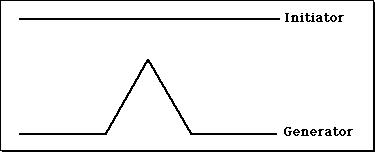
\includegraphics[scale=0.55]{images/koch1.png}
\caption{Initiator e generator per la curca di Koch}
\label{fig:k1}
\end{figure}

La regola può essere nuovamente applicata su ogni linea, così da andare a sostituirla ogni volta come fanno nel passaggio da \textit{initiator} a \textit{generator}. Il secondo livello è visibile in figura \ref{fig:k2}.

\begin{figure}[!ht]
\centering
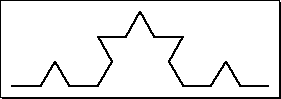
\includegraphics[scale=0.55]{images/koch2.png}
\caption{Livello 2 per la curca di Koch}
\label{fig:k2}
\end{figure}

\FloatBarrier

Una volta che la procedura è avviata può proseguire a piacimento. Il terzo e il quarto livello sono visibili nelle figure \ref{fig:k3} e \ref{fig:k4} rispettivamente.

\begin{figure}[!ht]
\centering
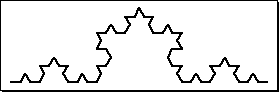
\includegraphics[scale=0.55]{images/koch3.png}
\caption{Livello 3 per la curca di Koch}
\label{fig:k3}
\end{figure}

\begin{figure}[!ht]
\centering
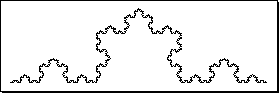
\includegraphics[scale=0.55]{images/koch4.png}
\caption{Livello 4 per la curca di Koch}
\label{fig:k4}
\end{figure}



\section{Iterated Function Systems}

Uno strumento matematico che si rivelerà fondamentale nella fase di decompressione delle immagini trattate con un metodo di compressione frattale è quello degli \emph{Iterated Function Systems}, che andiamo per questo motivo a descrivere qui.

Senza eccedere in formalità, definiamo un \emph{Iterated Function System} (IFS) come una collezione di trasformazioni contrattive $\{w_i : \mathbb{R}^2 \rightarrow \mathbb{R}^2 \}_{i=1,\ldots, n}$ che mappa il piano su se stesso. Questa collezione di trasformazioni definisce una mappa 

\[
W(\cdot) = \bigcup_{i=1}^{n} w_i(\cdot)
\]

Tale mappa è applicata ad insiemi di punti, ed il risultato è definito in questa maniera: dato un insieme di punti $S \in \mathbb{R}^2$, calcoliamo $w_i(S)$ per ogni $i$ (ovvero produciamo $i$ copie ridotte di $S$), e poi calcoliamo l'unione dei risultati (ovvero, mettiamo insieme tutte le copie ridotte), ottenendo così un nuovo insieme $S' = W(S)$.

$W$ così definito è una mappa tra sottoinsiemi di $\mathbb{R}^2$ (che d'ora in avanti per noi saranno ``immagini''), e gode di due importanti (e rilevanti per la compressione frattale) proprietà, che andiamo ad enunciare senza dimostrazione.

\begin{proprieta}
Se tutte le $w_i$ sono contrattive, allora $W$ è contrattiva in uno spazio di sottoinsiemi del piano.
\end{proprieta}

\begin{proprieta}
Fissata una mappa $W$, esiste una immagine $x_W$, chiamata \emph{attrattore per $W$}, tale che
\begin{itemize}
\item $W(x_W) = x_W$
\item data una qualunque immagine di partenza $S_0$, vale che 
\[x_W \equiv \lim_{n \rightarrow \infty} W^{n}(S_0) \]
ovvero l'applicazione ripetuta per $n$ volte di $W$ porta ad ottenere $x_W$, per $n$ sufficientemente grande, ed indipendentemente dalla scelta dell'immagine di partenza.
\item $x_W$ è unica. Se una qualsiasi immagine $S$ soddisfa $W(S) = S$, allora $S$ è l'attrattore per $W$.
\end{itemize}
\end{proprieta}

La seconda di queste proprietà è nota come \emph{Contractive Mapping Fixed-Point Theorem}.

\section{Self-similarity nelle immagini}

\subsection*{Immagini come oggetti matematici}

Per poter applicare la teoria degli \emph{IFS} alle immagini come comunemente le intendiamo (ovvero, in sostanza, matrici di pixels rappresentati  da 1 byte -- \emph{greyscale} -- oppure più di uno -- es. RBG --), è necessario formalizzare in qualche modo il concetto di ``immagine digitale'', cercando di inserirlo in un contesto matematico che ci consenta di manipolarla utilizzando di strumenti messi a disposizione dall'algebra. Per semplicità, ci limiteremo qui a considerare le immagini in \emph{grayscale} (un singolo canale di colore, l'intensità indicata con un numero da 0 a 255).

Consideriamo un'immagine in scala di grigi, memorizzata come matrice di pixel, 1 byte per ogni pixel. Non è difficile immaginare di poter rappresentare tale immagine utilizzando una funzione $f: \mathbb{R}^2 \rightarrow  \{1, 2, \ldots, 255 \}$, in modo tale che ad ogni pixel alle coordinate $(x, y)$ sia fatto corrispondere un punto $(x, y)$ nel piano, al quale a sua volta viene associata un'altezza $z$, che corrisponde al valore di grigio del pixel in questione. 

Ad esempio, ad un'immagine con il primo pixel in basso a sinistra avente livello di grigio 177, viene fatta corrispondere una funzione $f$ che, per quanto riguarda quel preciso punto, avrà $f(0,0) = 177$. Effettuando questa operazione su tutti i pixel dell'immagine originale, è possibile definire completamente $f$ su tutta la parte del piano di nostro interesse (e, in genere, si riduce per convenzione l'immagine ad avere dominio 
$[0, 1] \times [0,1]$). Nella figura qui sotto riportata si può vedere un esempio del risultato finale della procedura, applicata ad una immagine grayscale $128 \times 128$ pixels.

\begin{figure}[!ht]
\centering
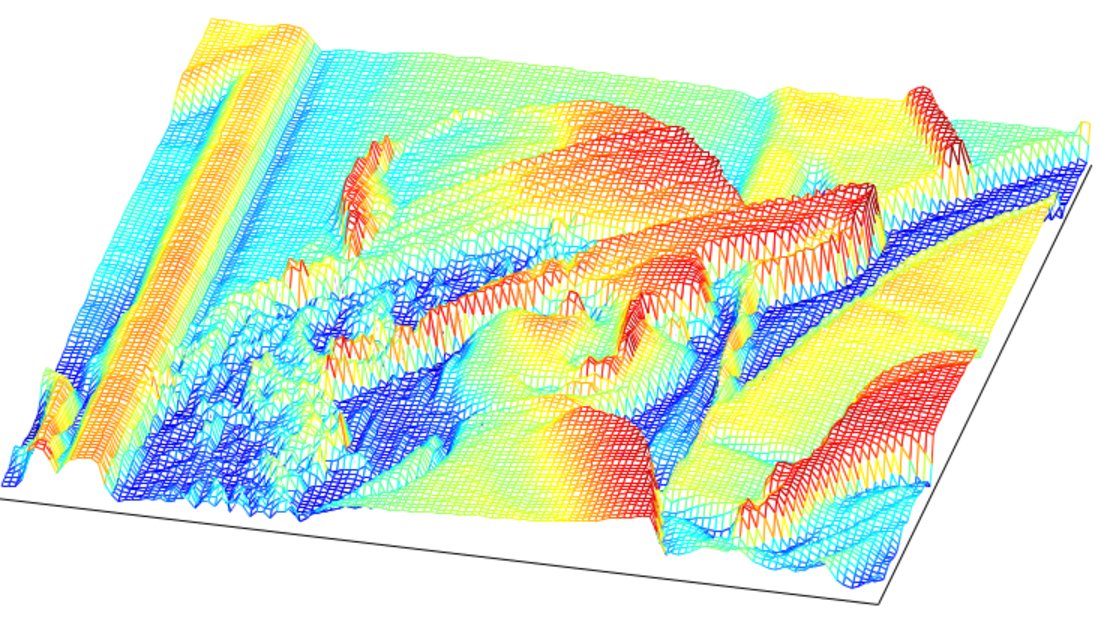
\includegraphics[scale=0.6]{images/lena-mash.pdf} 
\caption{lena grayscale, $128 \times 128$ pixels, trasformata in funzione $[0,1]^2 \rightarrow \{0,\ldots,255 \}$}
\end{figure}

La trasformazione descritta ci permette di ignorare l'aspetto ``visivo'' della modalità in cui una immagine è memorizzata, e ci consente di identificare una immagine con la funzione $f$ associata, su cui si andrà ad operare durante il procedimento di compressione.

\subsection*{Similarità tra due immagini}

Un secondo concetto che è necessario introdurre per poter operare sulle immagini durante il procedimento di compressione e decompressione è quello di ``distanza'' tra due immagini. La contrattività di una mappa $W$ (ovvero, intuitivamente, il fatto che essa rende le immagini più ``piccole'') può essere verificata solo se si ha a disposizione una qualche metrica sulla base della quale è possibile valutare la distanza tra due sottoinsiemi del piano (ovvero, nel nostro caso, due immagini).

Date due immagini $f, g$, definiamo la loro distanza $d(f, g)$, utilizzando la media quadratica, come

\[
d(f,s) = \sqrt{\int_{[0,1]^2} f(x,y) - g(x,y) \quad \text{d}x\text{d}y }
\]

La metrica ci fornisce una maniera di valutare la distanza tra due immagini pesando in maniera uniforme tutti i punti in esse contenuti.

\chapter{Aspetti Pratici ed una implementazione MATLAB}


\chapter{Test, benchmarks}


\end{document}
